\section{Performance Evaluation}
\label{sec:use-case}

This section evaluates the provisioned cluster through the SSB \citep{oneil2009star}. The central question is whether Spark's in-memory
processing outperforms Hive's disk-bound execution on the severely constrained
ARM hardware described in Section~\ref{sec:arch}, and whether explicit caching
yields further gains.

%%%%%%%%%%%%%%%%%%%%%%%%%%%%%%%%%%%%%%%%%%%%%%%%%%%%%%%%%%%%%%%%%%%%%%%%%%%%%%%%%%%%%%%%%%%%%%%%%%%%%%%%%%%%%%%%%%%
\subsection{Experimental Setup}

The benchmark was conducted on the cluster deployed under the
\texttt{data-science} installation profile
(Table~\ref{tab:comp-data-science}). Each of the four nodes is a
\texttt{VM.Standard.A1.Flex} instance with 1~OCPU and 6~GB of RAM. The active
services comprised HDFS, YARN, Hive Metastore, Hive Server~2, and Spark~3.

The SSB dataset was generated using the
\texttt{dbgen} tool provided with the benchmark suite. The flat-file sizes are
listed in Table~\ref{tab:ssb-dataset-sizes}; the largest file,
\texttt{lineorder.csv}, occupies 9.3~GB, producing a substantial I/O load for a
cluster with only three DataNodes and 6~GB of RAM per node. The generated CSV
files were first transferred to the master node's secondary block volume via
\texttt{scp}, then ingested into HDFS using \texttt{hdfs dfs~-put} as the HDFS
superuser. Staging directories were assigned YARN-compatible ownership and
permissions to allow both Hive and Spark to read the ingested data without
privilege escalation.

The cluster runs ODP version~1.2.2.0 on OL9 (aarch64), with
Hadoop~3.3.6, Spark~3.4.2, and Hive~3.1.3 as the primary engines; full
component versions are listed in Table~\ref{tab:odp-versions}. All services
execute on OpenJDK~1.8. HDFS was configured with the default replication factor
of~3 across the three DataNodes.

\begin{table}[htbp]
  \centering
  \caption{SSB dataset file sizes (scale factor SF\,=\,10).}
  \label{tab:ssb-dataset-sizes}
  \renewcommand{\arraystretch}{1.2}
  \begin{tabular}{ p{0.25\linewidth} p{0.15\linewidth} }
    \hline
    \textbf{File} & \textbf{Size} \\
    \hline
    lineorder.csv & 9.3 GB \\
    customer.csv  & 3.3 GB \\
    supplier.csv  & 211.7 MB \\
    part.csv      & 176.7 MB \\
    dwdate.csv    & 272.4 KB \\
    \hline
  \end{tabular}
\end{table}

The relational structure was registered in the Hive Metastore via the Beeline
CLI, connecting to HiveServer2 on a designated worker node. Five external
tables, \texttt{lineorder}, \texttt{customer}, \texttt{supplier},
\texttt{part}, and \texttt{dwdate}, were created using the
\texttt{OpenCSVSerde} deserialiser, with column types matching the SSB
specification. Because the tables are external, both Hive and Spark share a
single schema definition backed by the same HDFS data, ensuring that query
results are directly comparable across engines.

%%%%%%%%%%%%%%%%%%%%%%%%%%%%%%%%%%%%%%%%%%%%%%%%%%%%%%%%%%%%%%%%%%%%%%%%%%%%%%%%%%%%%%%%%%%%%%%%%%%%%%%%%%%%%%%%%%%
\subsection{Benchmark Protocol}

The evaluation comprised three processing configurations, each applied to the
full SSB query catalogue of 13 analytical queries (Listing~\ref{lst:ssb-queries}):

\begin{enumerate}
    \item \textbf{Hive (disk-bound):} Hive reads and writes sequential blocks
    to HDFS, operating within its native MapReduce-like execution model. This
    configuration tolerates severe memory limitations at the cost of processing
    speed.
    \item \textbf{Spark (no caching):} Spark reads data directly from
    HDFS without retaining any table in memory. This provides a baseline for
    Spark's performance under the same storage back-end as Hive.
    \item \textbf{Spark with caching:} Prior to querying, all SSB tables are
    cached in the Spark executors' memory. The cluster resources are explicitly
    constrained via \texttt{-{}-driver-memory} and \texttt{-{}-executor-memory}
    to prevent YARN container exhaustion.
\end{enumerate}

Each query was executed 10 times per configuration, yielding 390 individual
query runs in total (13 queries $\times$ 10 iterations $\times$ 3
configurations). All 10 iterations are included in the reported statistics; no
warm-up iterations were discarded.
Queries were submitted sequentially through shell scripts that wrap
each invocation and log wall-clock execution times to a
log file. The scripts were executed under \texttt{nohup} on the master node to
prevent SSH session timeouts, a practical necessity on free-tier instances whose
network connections are not guaranteed to remain stable over multi-hour runs.

The star schema and the 13 analytical queries are shown in
Figure~\ref{fig:ssb-schema} and Listing~\ref{lst:ssb-queries}, respectively.

\begin{lstlisting}[language=SQL, caption={SSB benchmark analytical queries.}, label={lst:ssb-queries}, frame=single, basicstyle=\ttfamily\scriptsize]
-- Q1.1
SELECT sum(lo_extendedprice*lo_discount) as revenue FROM ssb.lineorder JOIN ssb.dwdate ON lo_orderdate = d_datekey WHERE d_year = 1993 AND lo_discount between 1 and 3 AND lo_quantity < 25;

-- Q1.2
SELECT sum(lo_extendedprice*lo_discount) as revenue FROM ssb.lineorder JOIN ssb.dwdate ON lo_orderdate = d_datekey WHERE d_yearmonthnum = 199401 AND lo_discount between 4 and 6 AND lo_quantity between 26 and 35;

-- Q1.3
SELECT sum(lo_extendedprice*lo_discount) as revenue FROM ssb.lineorder JOIN ssb.dwdate ON lo_orderdate = d_datekey WHERE d_weeknuminyear = 6 AND d_year = 1994 AND lo_discount between 5 and 7 AND lo_quantity between 26 and 35;

-- Q2.1
SELECT sum(lo_revenue), d_year, p_brand FROM ssb.lineorder JOIN ssb.dwdate ON lo_orderdate = d_datekey JOIN ssb.part ON lo_partkey = p_partkey JOIN ssb.supplier ON lo_suppkey = s_suppkey WHERE p_category LIKE '%MFGR#12%' AND s_region LIKE '%AMERICA%' GROUP BY d_year, p_brand ORDER BY d_year, p_brand;

-- Q2.2
SELECT sum(lo_revenue), d_year, p_brand FROM ssb.lineorder JOIN ssb.dwdate ON lo_orderdate = d_datekey JOIN ssb.part ON lo_partkey = p_partkey JOIN ssb.supplier ON lo_suppkey = s_suppkey WHERE p_brand between 'MFGR#2221' and 'MFGR#2228' AND s_region LIKE '%ASIA%' GROUP BY d_year, p_brand ORDER BY d_year, p_brand;

-- Q2.3
SELECT sum(lo_revenue), d_year, p_brand FROM ssb.lineorder JOIN ssb.dwdate ON lo_orderdate = d_datekey JOIN ssb.part ON lo_partkey = p_partkey JOIN ssb.supplier ON lo_suppkey = s_suppkey WHERE p_brand LIKE '%MFGR#2221%' AND s_region LIKE '%EUROPE%' GROUP BY d_year, p_brand ORDER BY d_year, p_brand;

-- Q3.1
SELECT c_nation, s_nation, d_year, sum(lo_revenue) as revenue FROM ssb.lineorder JOIN ssb.customer ON lo_custkey = c_custkey JOIN ssb.supplier ON lo_suppkey = s_suppkey JOIN ssb.dwdate ON lo_orderdate = d_datekey WHERE c_region LIKE '%ASIA%' AND s_region LIKE '%ASIA%' AND d_year >= 1992 AND d_year <= 1997 GROUP BY c_nation, s_nation, d_year ORDER BY d_year asc, revenue desc;

-- Q3.2
SELECT c_city, s_city, d_year, sum(lo_revenue) as revenue FROM ssb.lineorder JOIN ssb.customer ON lo_custkey = c_custkey JOIN ssb.supplier ON lo_suppkey = s_suppkey JOIN ssb.dwdate ON lo_orderdate = d_datekey WHERE c_nation LIKE '%UNITED STATES%' AND s_nation LIKE '%UNITED STATES%' AND d_year >= 1992 AND d_year <= 1997 GROUP BY c_city, s_city, d_year ORDER BY d_year asc, revenue desc;

-- Q3.3
SELECT c_city, s_city, d_year, sum(lo_revenue) as revenue FROM ssb.lineorder JOIN ssb.customer ON lo_custkey = c_custkey JOIN ssb.supplier ON lo_suppkey = s_suppkey JOIN ssb.dwdate ON lo_orderdate = d_datekey WHERE (c_city LIKE '%UNITED KI1%' or c_city LIKE '%UNITED KI5%') AND (s_city LIKE '%UNITED KI1%' or s_city LIKE '%UNITED KI5%') AND d_year >= 1992 AND d_year <= 1997 GROUP BY c_city, s_city, d_year ORDER BY d_year asc, revenue desc;

-- Q3.4
SELECT c_city, s_city, d_year, sum(lo_revenue) as revenue FROM ssb.lineorder JOIN ssb.customer ON lo_custkey = c_custkey JOIN ssb.supplier ON lo_suppkey = s_suppkey JOIN ssb.dwdate ON lo_orderdate = d_datekey WHERE (c_city LIKE '%UNITED KI1%' or c_city LIKE '%UNITED KI5%') AND (s_city LIKE '%UNITED KI1%' or s_city LIKE '%UNITED KI5%') AND d_yearmonth LIKE '%Dec1997%' GROUP BY c_city, s_city, d_year ORDER BY d_year asc, revenue desc;

-- Q4.1
SELECT d_year, c_nation, sum(lo_revenue - lo_supplycost) as profit FROM ssb.lineorder JOIN ssb.dwdate ON lo_orderdate = d_datekey JOIN ssb.customer ON lo_custkey = c_custkey JOIN ssb.supplier ON lo_suppkey = s_suppkey JOIN ssb.part ON lo_partkey = p_partkey WHERE c_region LIKE '%AMERICA%' AND s_region LIKE '%AMERICA%' AND (p_mfgr LIKE '%MFGR#1%' or p_mfgr LIKE '%MFGR#2%') GROUP BY d_year, c_nation ORDER BY d_year, c_nation;

-- Q4.2
SELECT d_year, s_nation, p_category, sum(lo_revenue - lo_supplycost) as profit FROM ssb.lineorder JOIN ssb.dwdate ON lo_orderdate = d_datekey JOIN ssb.customer ON lo_custkey = c_custkey JOIN ssb.supplier ON lo_suppkey = s_suppkey JOIN ssb.part ON lo_partkey = p_partkey WHERE c_region LIKE '%AMERICA%' AND s_region LIKE '%AMERICA%' AND (d_year = 1997 or d_year = 1998) AND (p_mfgr LIKE '%MFGR#1%' or p_mfgr LIKE '%MFGR#2%') GROUP BY d_year, s_nation, p_category ORDER BY d_year, s_nation, p_category;

-- Q4.3
SELECT d_year, s_city, p_brand, sum(lo_revenue - lo_supplycost) as profit FROM ssb.lineorder JOIN ssb.dwdate ON lo_orderdate = d_datekey JOIN ssb.customer ON lo_custkey = c_custkey JOIN ssb.supplier ON lo_suppkey = s_suppkey JOIN ssb.part ON lo_partkey = p_partkey WHERE c_region LIKE '%AMERICA%' AND s_nation LIKE '%UNITED STATES%' AND (d_year = 1997 or d_year = 1998) AND p_category LIKE '%MFGR#14%' GROUP BY d_year, s_city, p_brand ORDER BY d_year, s_city, p_brand;
\end{lstlisting}

%%%%%%%%%%%%%%%%%%%%%%%%%%%%%%%%%%%%%%%%%%%%%%%%%%%%%%%%%%%%%%%%%%%%%%%%%%%%%%%%%%%%%%%%%%%%%%%%%%%%%%%%%%%%%%%%%%%
\subsection{Results and Analysis}

\begin{figure}[htbp]
    \centering
    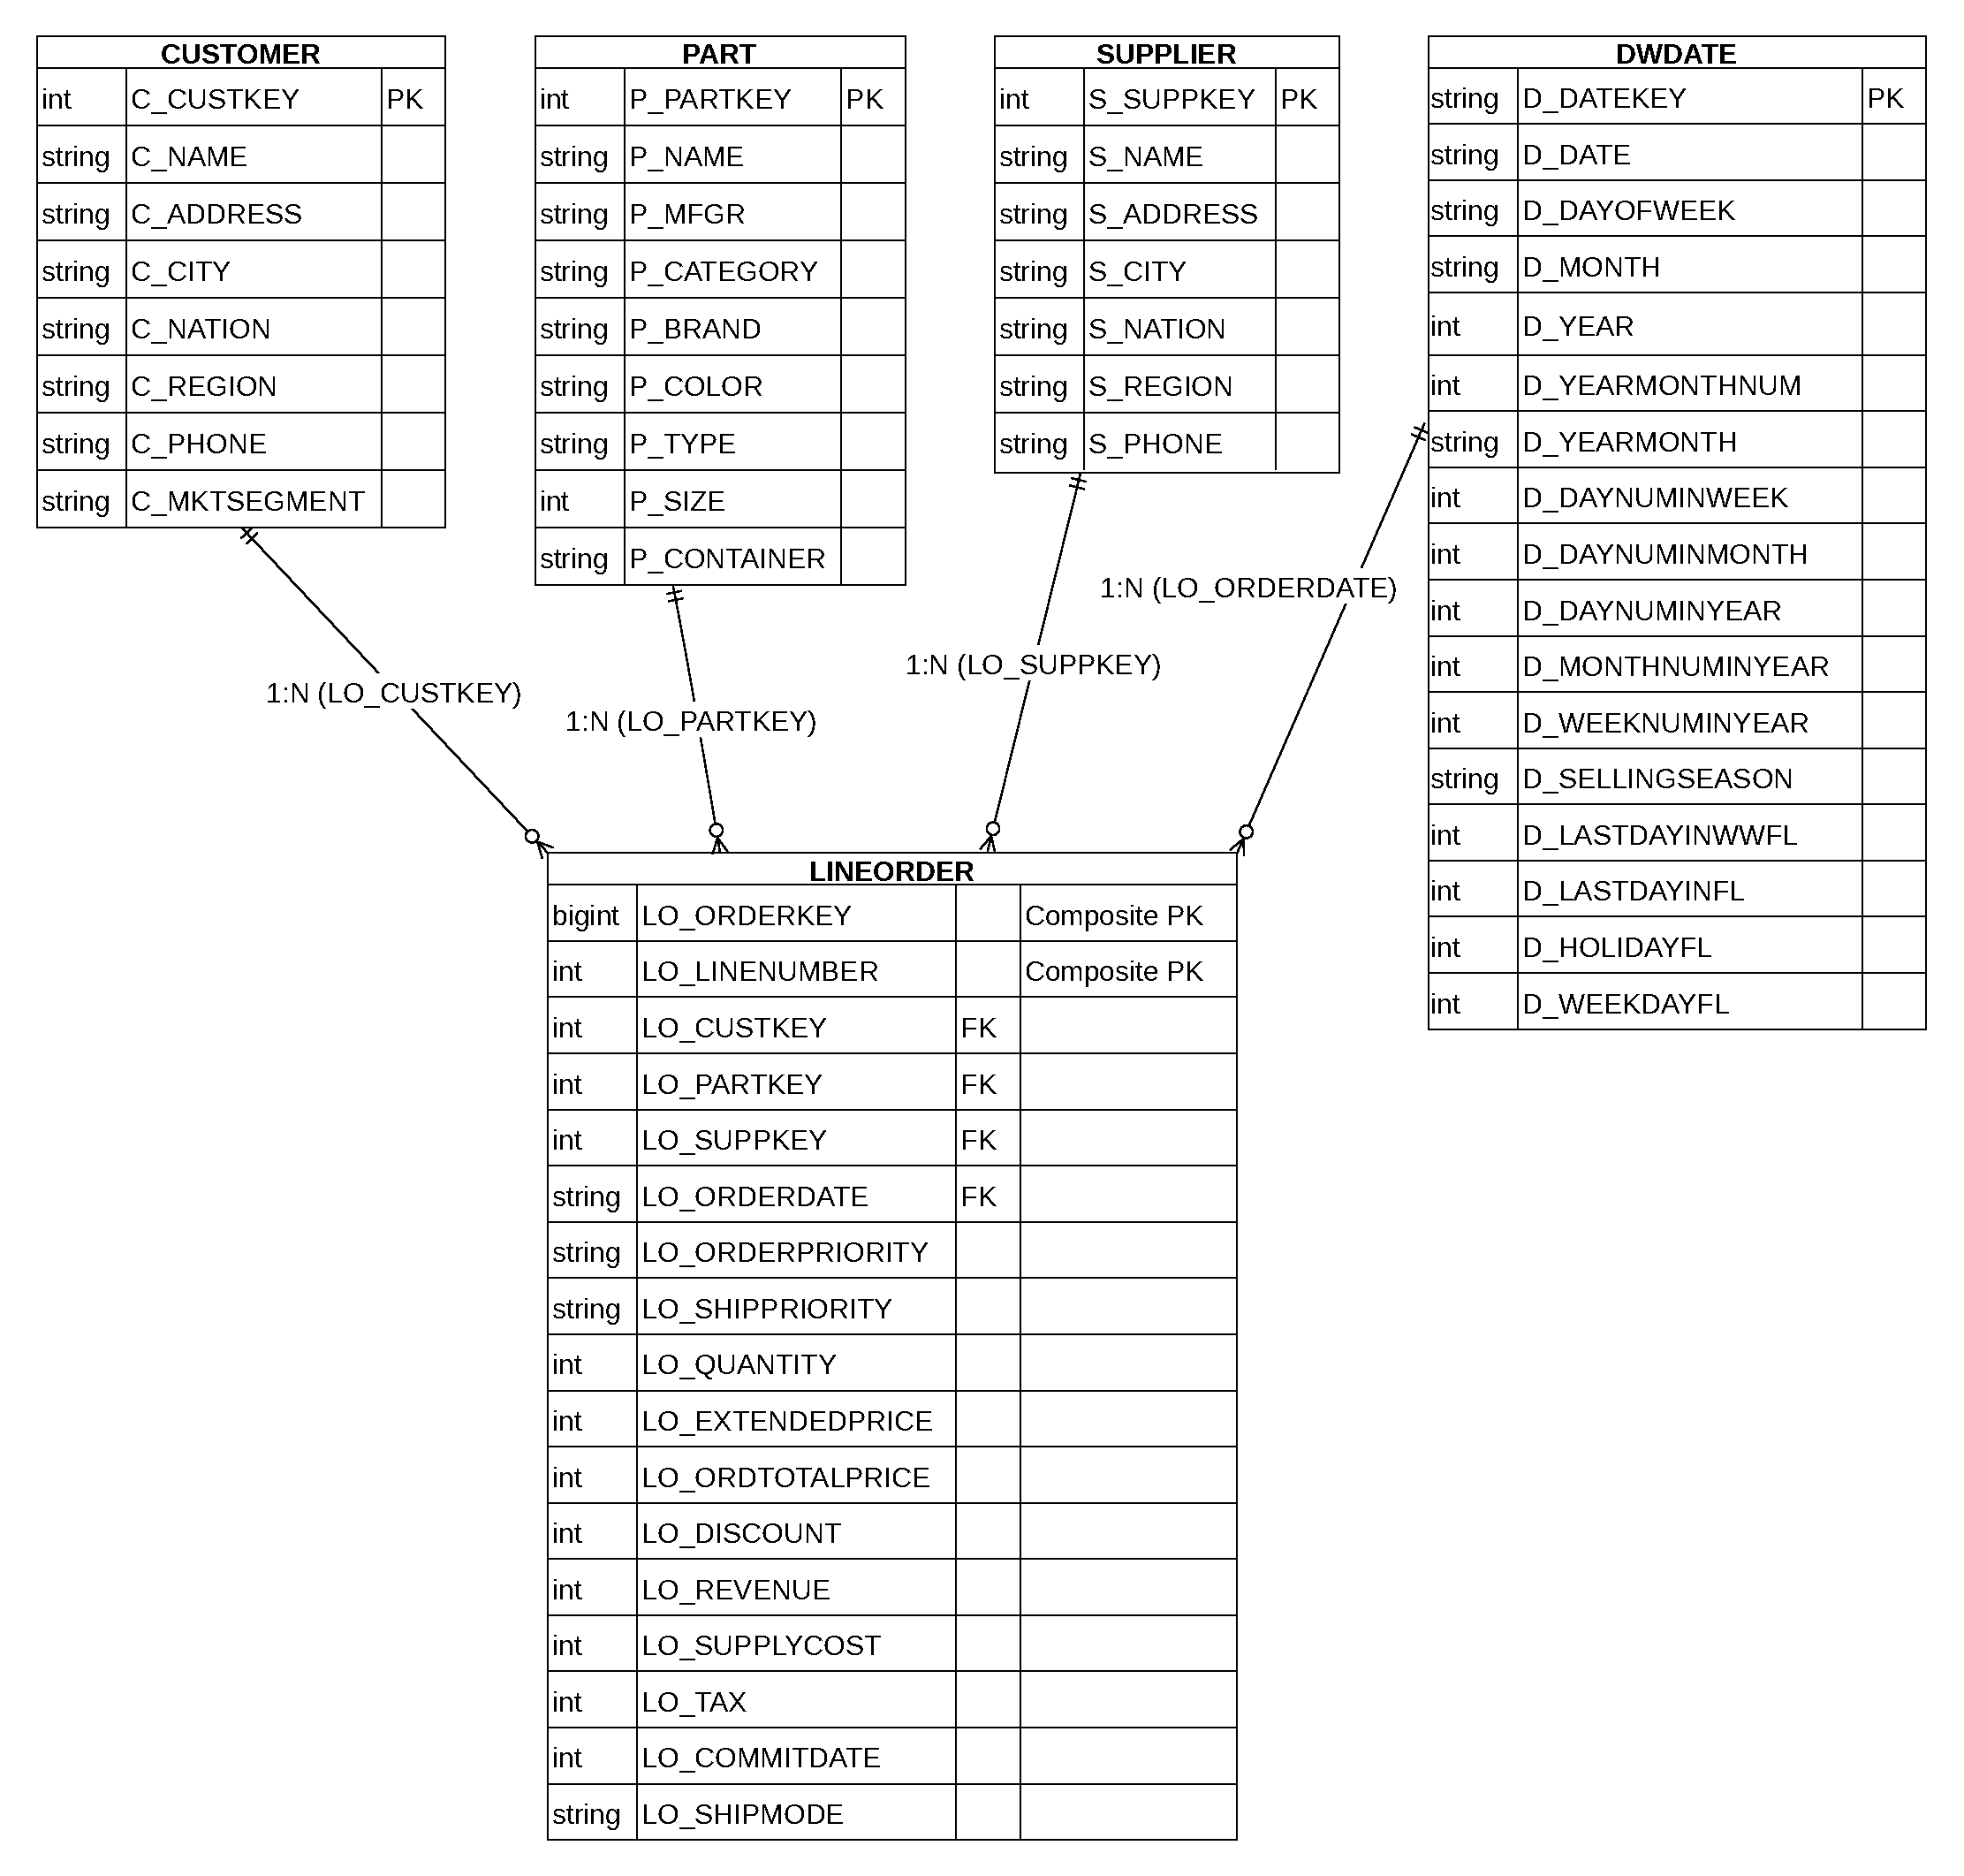
\includegraphics[width=\linewidth]{content/assets/schema.pdf}
    \caption{SSB star schema entity-relationship diagram.}
    \label{fig:ssb-schema}
\end{figure}

\begin{figure}[htbp]
    \centering
    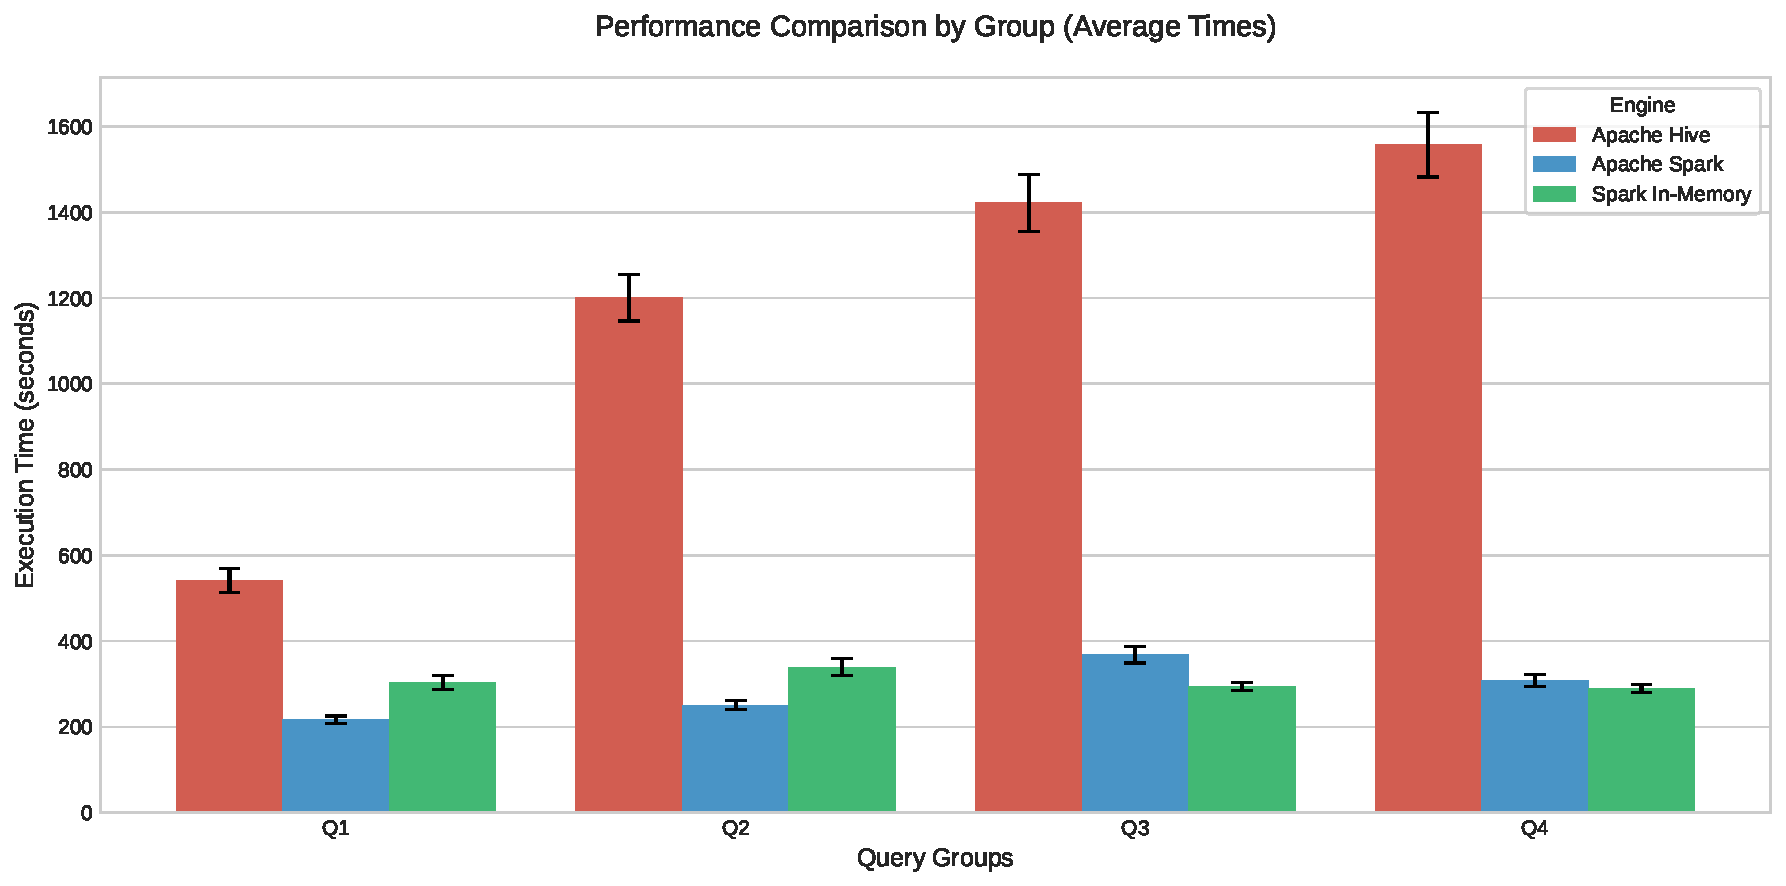
\includegraphics[width=\linewidth]{content/assets/graphic-group.pdf}
    \caption{Group-level mean query execution times (seconds) for the four SSB
             complexity bands (Q1: Q1.1--Q1.3; Q2: Q2.1--Q2.3; Q3: Q3.1--Q3.4;
             Q4: Q4.1--Q4.3), comparing Hive, Spark without cache, and Spark with
             caching. Each bar aggregates the per-query means within the group.
             Error bars illustrate synthetic dispersion around those means and do
             not match the empirical standard deviations in
             Table~\ref{tab:benchmark-results}.}
    \label{fig:query-execution-time-comparison}
\end{figure}

Table~\ref{tab:benchmark-results} reports the mean execution time and standard
deviation \emph{for each individual query} across the three configurations,
computed from the full set of 10 measured iterations per query--configuration
pair; no outliers were removed. Figure~\ref{fig:query-execution-time-comparison}
provides a complementary \emph{group-level} view: the same 13 queries are rolled
into the four bands used later in this subsection, so each cluster of bars
summarises how the three engines behave on average for that band. The
following points highlight how to read the chart alongside the table.

\begin{itemize}
    \item \textbf{Group~Q1} (single-join queries Q1.1--Q1.3): Hive clearly
    dominates the bar heights; Spark without cache is much lower; Spark with
    cache typically sits between the two or above uncached Spark, matching the
    later observation that caching adds overhead on the lightest queries when
    the large fact table cannot be held entirely in memory.
    \item \textbf{Group~Q2} (Q2.1--Q2.3 with \texttt{part} and
    \texttt{supplier}): Hive remains the slowest configuration; Spark without
    cache delivers the largest relative drop in bar height within the group;
    cached Spark again tends to exceed uncached Spark, signalling that the
    cache path still pays shuffle and spill costs under the same memory ceiling.
    \item \textbf{Group~Q3} (Q3.1--Q3.4 with \texttt{customer} and
    \texttt{supplier}): absolute bar levels rise relative to Q1--Q2, yet Spark
    stays well below Hive; the relative ordering between uncached and cached
    Spark varies across the constituent queries, so the grouped bars summarise
    a mix of modest penalties and visible gains that Table~\ref{tab:benchmark-results}
    resolves at per-query granularity.
    \item \textbf{Group~Q4} (profit queries Q4.1--Q4.3): Hive reaches the highest
    averages in the figure; Spark still lowers execution substantially; cached
    Spark can approach or beat uncached Spark where partial dimension caching
    amortises the join workload, which is easier to see in the table for Q3.2
    and neighbouring queries than in the aggregate bar alone.
    \item \textbf{Across groups:} in this aggregated view, mean Hive time
    increases from Q1 through Q4 while Spark remains comparatively flat, so the
    visual gap between Hive and Spark widens with join complexity, consistent
    with the quantitative group analysis below, even though the chart does not
    depict one bar per query.
\end{itemize}

\begin{table}[htbp]
  \centering
  \caption{Mean query execution time in seconds, with standard deviation in
           parentheses, over 10 iterations per configuration.}
  \label{tab:benchmark-results}
  \renewcommand{\arraystretch}{1.15}
  \small
  \begin{tabular}{@{} l c c c @{}}
    \hline
    \textbf{Query} & \textbf{Hive} & \textbf{Spark} & \textbf{Spark+Cache} \\
    \hline
    Q1.1  &  561.1\,\pm 23.0 & 203.0\,\phantom{0}\pm 9.7 & 298.7\,\pm 11.7 \\
    Q1.2 &  541.5\,\pm 14.9 & 259.9\,\pm 11.1 & 311.0\,\pm 11.9 \\
    Q1.3  &  557.0\,\pm 42.8 & 204.9\,\pm 12.4 & 295.3\,\pm 11.7 \\
    Q2.1  & 1{,}120.2\,\pm 44.0 & 257.8\,\phantom{0}\pm 6.1 & 354.2\,\pm 14.4 \\
    Q2.2  & 1{,}519.3\,\pm 65.3 & 238.2\,\pm 10.8 & 334.0\,\pm 20.6 \\
    Q2.3  &  959.4\,\pm 59.9 & 252.5\,\pm 13.1 & 336.2\,\pm 22.9 \\
    Q3.1  & 1{,}175.1\,\pm 62.2 & 318.3\,\pm 20.3 & 290.0\,\phantom{0}\pm 9.2 \\
    Q3.2  & 1{,}871.5\,\pm 87.3 & 574.8\,\pm 27.5 & 277.7\,\pm 14.4 \\
    Q3.3  & 1{,}785.5\,\pm 77.8 & 288.2\,\pm 17.1 & 338.1\,\pm 15.2 \\
    Q3.4  &  884.4\,\pm 26.7 & 278.3\,\pm 16.7 & 268.0\,\pm 14.8 \\
    Q4.1  & 2{,}459.1\,\pm 77.9 & 347.2\,\pm 21.1 & 339.4\,\pm 14.6 \\
    Q4.2  & 1{,}326.0\,\pm 75.7 & 279.0\,\pm 10.3 & 258.2\,\pm 12.1 \\
    Q4.3  &  881.0\,\pm 45.1 & 288.1\,\phantom{0}\pm 6.2 & 253.8\,\pm 16.5 \\
    \hline
  \end{tabular}
\end{table}

\subsubsection{Hive, Spark, and caching}

Across all 13 queries, Spark reduced mean
execution time relative to Hive by approximately \PaperHSRedPctMeanAgg\% when
averaging over all queries, with per-query reductions ranging from
\PaperHSRedPctMin\% to \PaperHSRedPctMax\%. The SSB query catalogue is
structured into four groups of increasing join complexity. The first group
(Q1.1, Q1.2, Q1.3) performs single-join aggregations over \texttt{lineorder} and
\texttt{dwdate}; Hive averages \PaperExpHSGOneMeanHive~seconds per query whereas Spark averages
\PaperExpHSGOneMeanSpark~seconds, corresponding to approximately \PaperExpHSGOneRedPct\% less time than Hive for this group.
The second group (Q2.1--Q2.3) adds
three-way and four-way joins involving \texttt{part} and \texttt{supplier},
and the gap widens: Hive averages \PaperExpHSGTwoMeanHive~seconds against Spark's
\PaperExpHSGTwoMeanSpark~seconds (approximately \PaperExpHSGTwoRedPct\% reduction relative to Hive).
The third group (Q3.1--Q3.4) joins \texttt{customer} and
\texttt{supplier} dimensions with progressively tighter filters; Hive
averages \PaperExpHSGThreeMeanHive~seconds while Spark averages \PaperExpHSGThreeMeanSpark~seconds (approximately \PaperExpHSGThreeRedPct\% reduction relative to Hive).
The fourth group
(Q4.1--Q4.3) computes profit metrics over four-way joins and exhibits the
largest relative margin between Hive and Spark (approximately \PaperExpHSGFourRedPct\% less time than Hive on average for this group), with Hive averaging \PaperExpHSGFourMeanHive~seconds versus Spark's
\PaperExpHSGFourMeanSpark~seconds. All differences are consistent across the 10 iterations, as
indicated by the relatively low standard deviations.

The comparison between the two
Spark configurations is less straightforward. For the simpler two-join queries
(Q1.1, Q1.2, Q1.3), the cached configuration was consistently slower, increasing latency by approximately
\PaperExpCacheQOneOverMinPct\% to \PaperExpCacheQOneOverMaxPct\% relative to uncached Spark.
A similar penalty
applies to the three-way and four-way join queries Q2.1--Q2.3, where caching added approximately
\PaperExpCacheQTwoOverMinPct\% to \PaperExpCacheQTwoOverMaxPct\%, and to Q3.3, where the overhead was approximately \PaperExpCacheQThreeThreeOverPct\%. In
all of these cases, the penalty stems from the attempt to cache the 9.3~GB
\texttt{lineorder} fact table into the cluster's limited memory: the table
cannot be fully cached, and the resulting shuffle and disk spill costs penalise
execution without conferring a commensurate read-back benefit.

For the remaining queries involving tighter filters and higher-cardinality
joins (Q3.1, Q3.2, Q3.4--Q4.3), partial caching of the smaller dimension tables
yielded a net benefit. The largest gain appeared in Q3.2, where caching reduced
mean execution time relative to uncached Spark by approximately \PaperQThreeTwoCacheImprovementPct\%;
Q3.1 improved by approximately \PaperExpQThreeOneCacheGainPct\%, and Q3.4 through Q4.3
showed gains of approximately \PaperExpCacheQThreeFourQFourThreeGainMinPct\% to \PaperExpCacheQThreeFourQFourThreeGainMaxPct\%. Averaged across all 13 queries,
however, the cached configuration was \PaperCacheVsSparkMeanPenaltyPct\% slower than uncached Spark,
indicating that caching is counterproductive under these memory constraints
unless the query complexity is sufficient to amortise the overhead.

\subsubsection{Resource limits and discussion}

The restriction to two executors reflects a hard CPU constraint, not merely a 
memory limitation. The blueprint configures
one virtual core per NodeManager, and three of the four nodes act as
NodeManagers, yielding three YARN containers in total. Because the Spark
Application Master claims one container, at most two remain available for
executors. Any attempt to allocate a third executor would cause a resource
deadlock. Each executor receives 1~GB of heap memory plus a 256~MB overhead
allocation; the driver is limited to 512~MB. These values were chosen to
prevent YARN from killing containers when the operating system and other Hadoop
daemons (HDFS DataNode, NodeManager) compete for the same 6~GB of physical RAM
on each node.

A methodological caveat applies to the comparison between the two Spark
configurations. The ``standard'' invocation relies on YARN's default resource
allocation, whereas the ``cached'' configuration explicitly sets
\texttt{driver-memory}, \texttt{executor-memory},
\texttt{spark.memory.fraction} (0.8 versus the default~0.6), and
\texttt{spark.sql.shuffle.partitions} (48 versus the default~200). The
observed performance difference therefore reflects not only the effect of
caching but also the change in memory allocation and shuffle behaviour.
Isolating the caching effect alone would require a run with identical resource
parameters but without the cache directives; such a run was not performed in
this study. This confound is revisited in the limitations discussed in
Section~\ref{sec:conclusion}.

Despite these constraints, all 390 query executions (13 queries $\times$ 10
iterations $\times$ 3 configurations) completed without unrecoverable failures.
Spark fell back to disk when in-memory caching could not be
sustained, confirming the operational stability of the platform under
prolonged stress.

These results can be situated within the broader
findings of prior ARM benchmarking studies. \citet{loghin2015performance}
observed that I/O-bound workloads are less sensitive to processor
micro-architecture than CPU-bound ones; the SSB queries used here are
predominantly I/O-bound, reading large fact tables from HDFS, which may
explain why the ARM instances sustain acceptable Spark throughput despite
being limited to a single virtual core per node. \citet{8287751} reported
favourable cost-efficiency ratios for Hadoop and Spark on commodity ARM64
servers with substantially greater per-node resources. The present study
extends that observation to the extreme lower bound of the resource
spectrum: a cluster where each node has only 1~vCPU and 6~GB of RAM, yet
Spark still outperforms Hive by factors of 2.5$\times$ to 5$\times$
depending on query complexity. The caching analysis, however, reveals a
boundary condition not explored in earlier work: when the largest table
exceeds available memory and the executor count is fixed at two, the
overhead of attempted caching outweighs its benefits for the majority of
queries. This suggests that caching strategies validated on larger clusters
cannot be directly transferred to free-tier-class hardware without careful
tuning of memory allocation parameters.
